\section{Axes}

\subsection{WebMGA 2.0 Implementation}
\begin{figure}
  \begin{center}
    \begin{subfigure}{0.4\textwidth}
      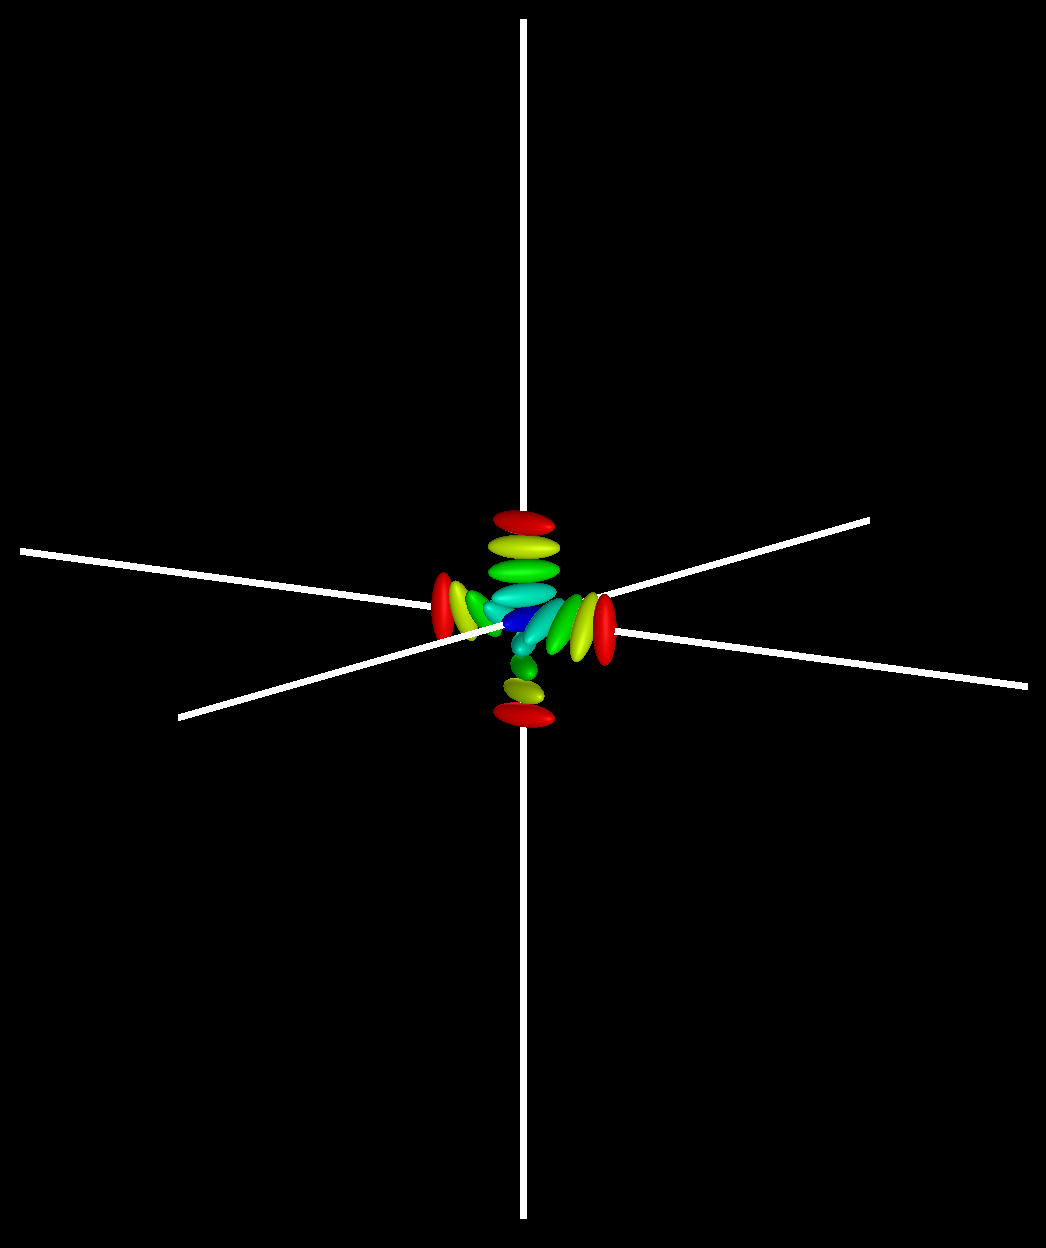
\includegraphics[width=\linewidth]{assets/images/axes/2_no_colour}
      \caption{Colour disabled.}
      \label{fig:original_axes_no_colour}
    \end{subfigure}
    \begin{subfigure}{0.4\textwidth}
      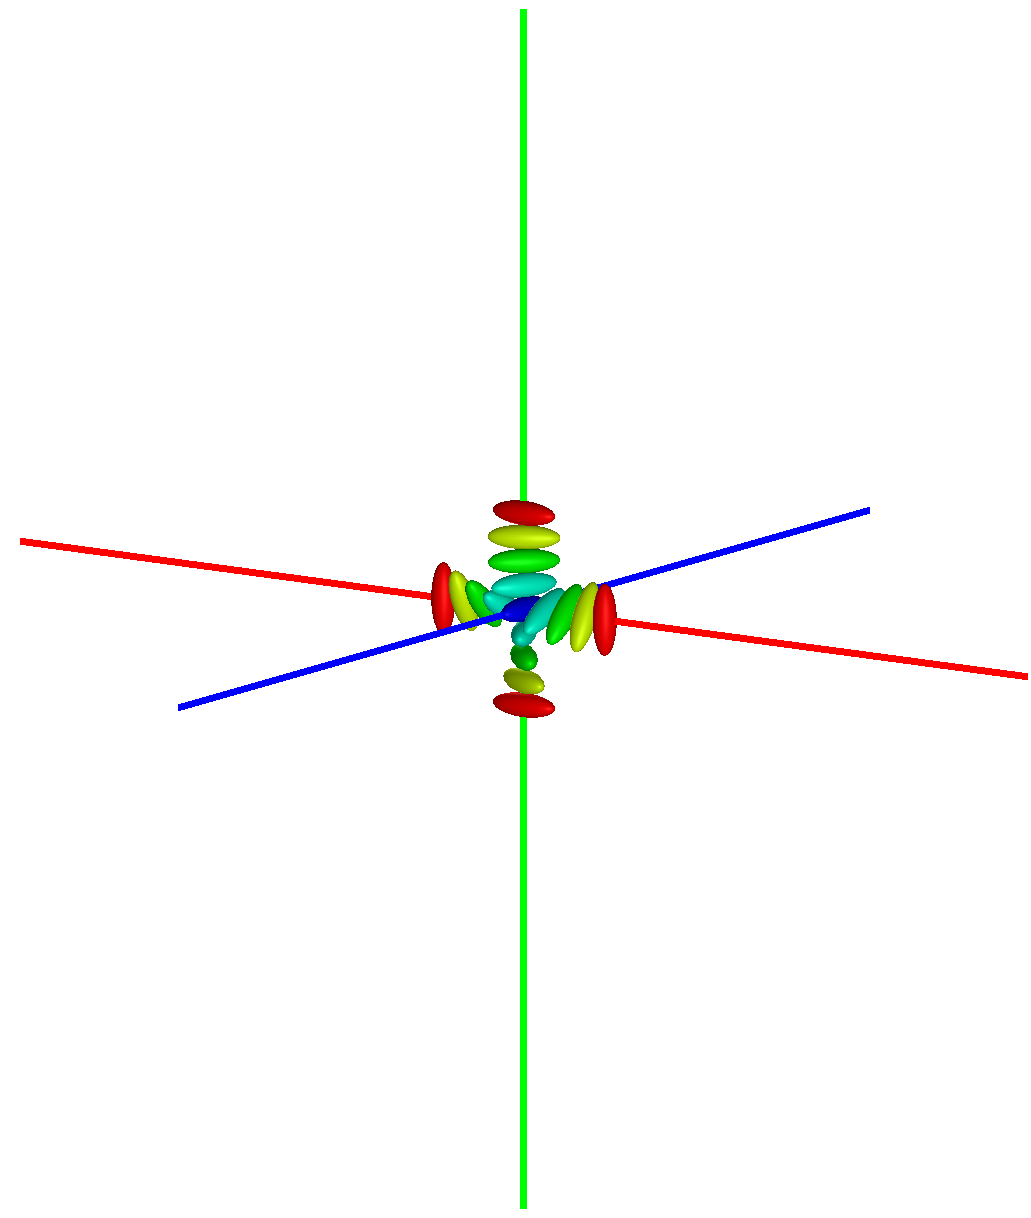
\includegraphics[width=\linewidth]{assets/images/axes/2_colour}
      \caption{Colour enabled.}
      \label{fig:original_axes_colour}
    \end{subfigure}
    \begin{subfigure}{0.4\textwidth}
      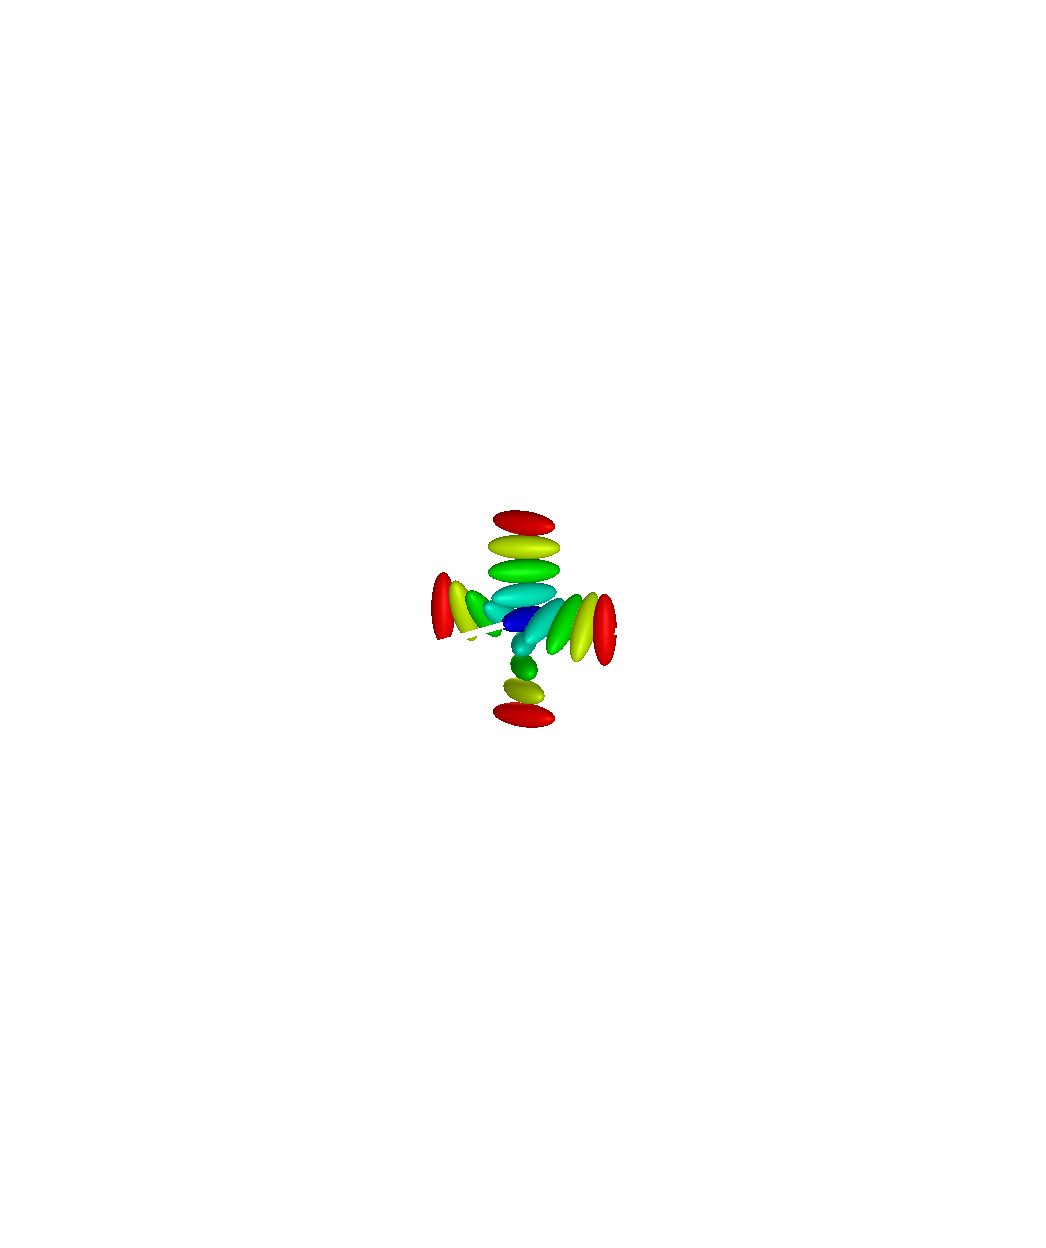
\includegraphics[width=\linewidth]{assets/images/axes/2_no_colour_bad}
      \caption{Colour disabled (light mode).}
      \label{fig:original_axes_no_colour_bad}
    \end{subfigure}
    \begin{subfigure}{0.4\textwidth}
      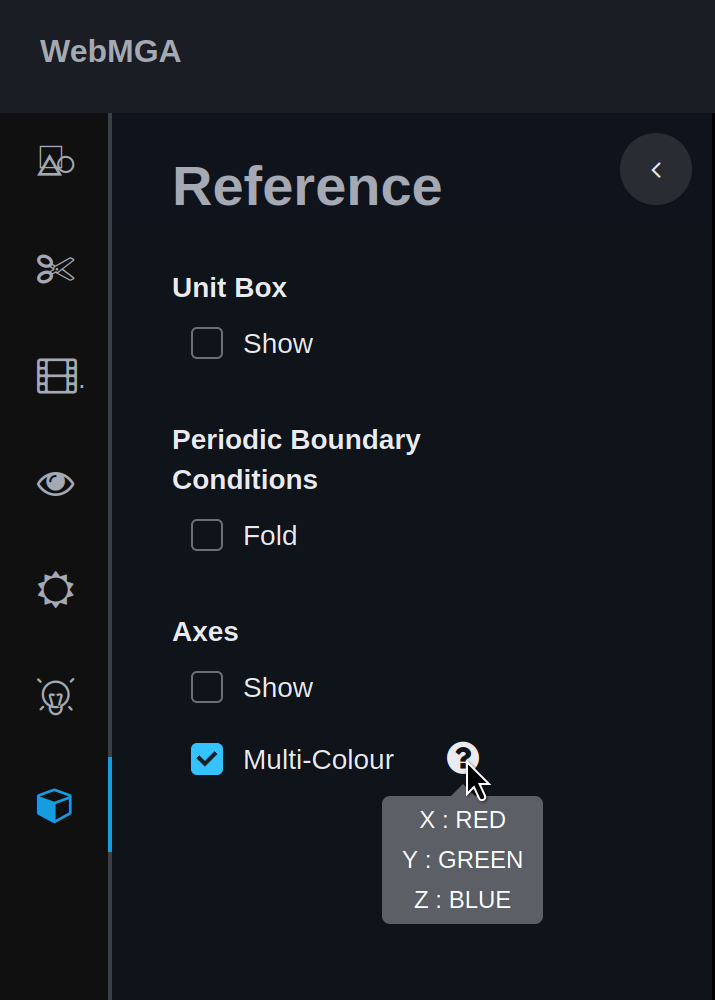
\includegraphics[width=\linewidth]{assets/images/axes/2_gui}
      \caption{GUI controls.}
      \label{fig:original_axes_controls}
    \end{subfigure} 
  \end{center}
  \caption{Axes in WebMGA 2.0.}
  \label{fig:original_axes}
\end{figure}

In WebMGA 2.0, the 3D axes are displayed as shown in \cref{fig:original_axes_no_colour,fig:original_axes_colour}, and controlled through the user interface as shown in \cref{fig:original_axes_controls} (visibility and colour toggles).

Axes take the form of three lines of fixed lengths in the $x$, $y$, and $z$ directions. Each line's midpoint is the lab frame coordinate $(0, 0, 0)$, where all axes meet. Axes extend in both positive and negative directions. They are not shown by default and, when first enabled, are uncoloured. When coloured, the $x$ axis is red, the $y$ axis is green, and the $z$ axis is blue.

Visibility is toggled using the ``Show'' button and colour is toggled with the ``Multi-Colour'' button. A question mark icon is next to the ``Multi-Colour'' which shows a tooltip when hovered specifying the axis colour scheme.

\subsection{WebMGA 2.0 Bugs}
\begin{figure}
  \begin{center}
    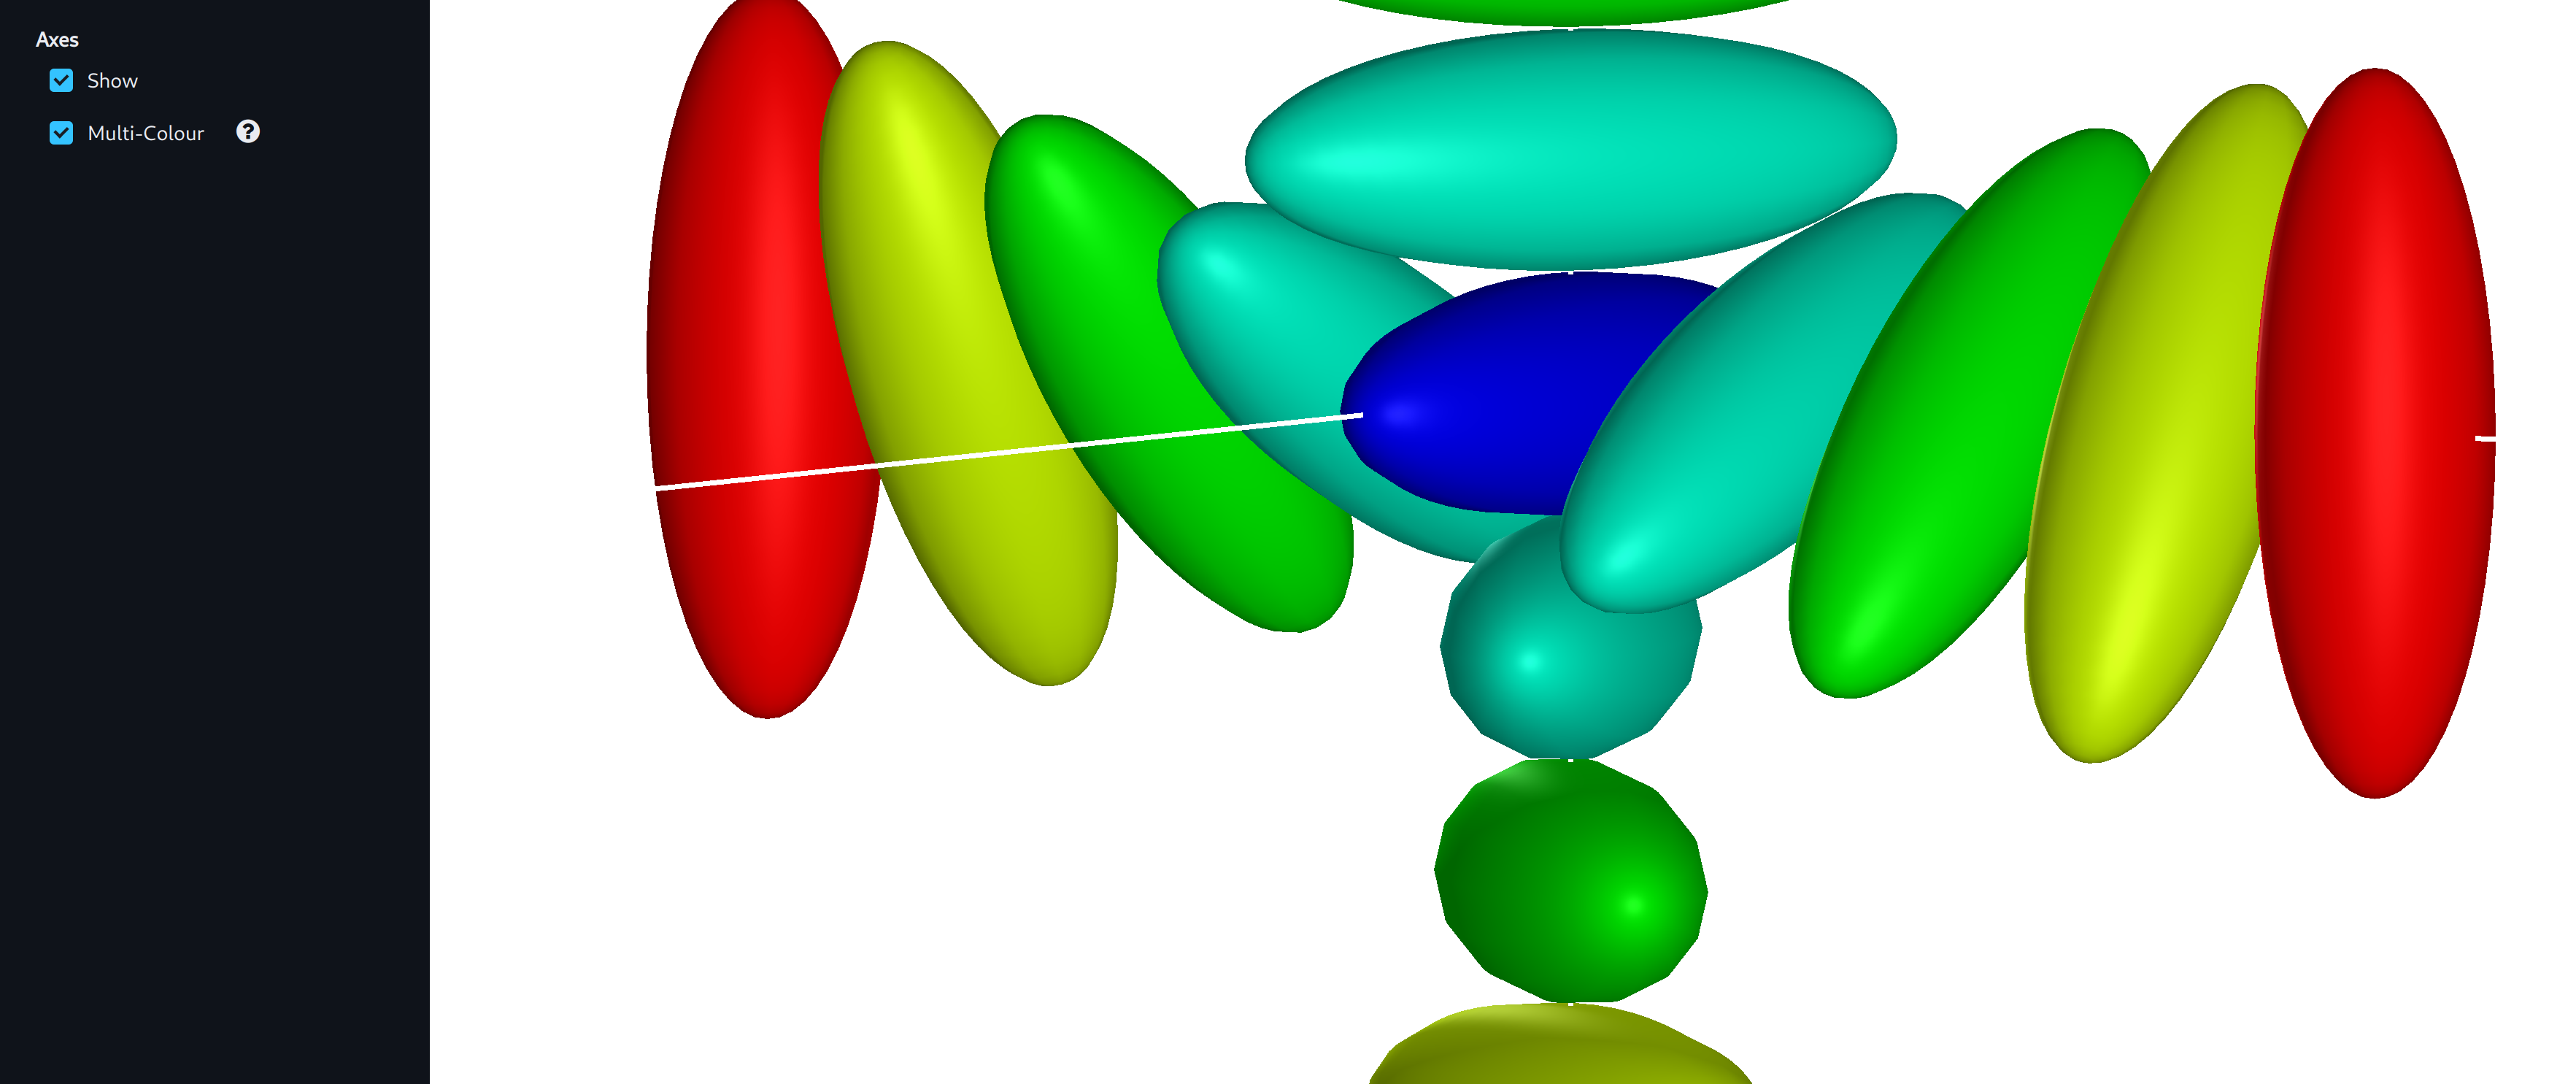
\includegraphics[width=\linewidth]{assets/images/axes/2_bug}
    \caption{\centering Bug where axes are not coloured despite the ``Multi-Colour'' toggle being enabled when axes are first enabled.}
    \label{fig:original_bug}
  \end{center}
\end{figure}

When the axes are toggled to visible for the first time, if the ``Multi-Colour'' toggle has not been interacted with first, the axes will be uncoloured, despite the ``Multi-Colour'' toggle being enabled by default. This is shown in \cref{fig:original_bug}. To enable colour for the first time, the ``Multi-Colour'' toggle must be disabled and then re-enabled.

When the environment is set to light mode (white background) with coloured axes disabled, the axes become difficult to view since they retain a white colour as default, blending into the background as shown in \cref{fig:original_axes_no_colour_bad}.

\subsection{Improvement Goals}
\begin{itemize}
  \item Axes are unlabelled
    \begin{itemize}
      \item Axes should be changed to extend only in the positive direction
    \end{itemize}
  \item Director(see \cref{pbc_explain} for definition) is not shown
    \begin{itemize}
      \item An additional line should be shown indicating director direction
    \end{itemize}
  \item Colours should be labelled or meaningful
    \begin{itemize}
      \item Colour axes according to angle with director (as in \cref{colour_director})
    \end{itemize}
  \item Axes should not be obscured
    \begin{itemize}
      \item Place axes in screen corner rather than centre
    \end{itemize}
  \item Axes should be clearly distinguishable
    \begin{itemize}
      \item Ensure axes retain contrast with background under light and dark views
    \end{itemize}
\end{itemize}

\subsection{WebMGA 3.0 Implementation}
\subsubsection{Axes Positions}
\label{axes_positions_sec}
The existing implementation was found to be needlessly convoluted so was largely stripped out. For example, coloured and uncoloured axes were implemented entirely separately, resulting in a large amount of duplicated code and convoluted logic flow. The bug identified in WebMGA 2.0 regarding uncoloured axes showing with ``Multi-Colour'' enabled, for example, was found to occur due to incorrect colour object initialisation, meaning what should be ``Multi-Colour'' axes showed as uncoloured since the colours are not defined when these lines are loaded the very first time.

In the new axes code, they are simply defined in terms of an axes centre point, three axes vectors, and an axis length scale. The axes vectors are handled in the lab frame so are trivially defines as $x=(1,0,0)$, $y=(0,1,0)$, and $z=(0,0,1)$.

Since the axes centre needs to remain in a fixed position on screen at all times, it needs to be defined relative to the camera. Three.js provides a method on any world object which converts from object relative coordinates to the lab frame, so this is used to trivially place the axes centre into the lab frame as required. Since this relationship changes when an object, in this case the camera, moves, the axes centre must therefore be redefined on any camera movement. This process also does not account for changes to intrinsic camera properties, importantly camera zoom. The axes therefore need to be scaled proportionally to the camera's zoom level on any zoom change.

Using the lab frame centre point and the axes vectors and scales, axis lines are trivially defined as,

\begin{equation}
  l_0=c\label{axes_vector_1}
\end{equation}
\begin{equation}
  l_1=c+szv\label{axes_vector_2}
\end{equation}
where $l_0$ and $l_1$ are the axis line start and end, $c$ is the axes centre, $v$ is the axis vector, $s$ is the axis scale factor, and $z$ is the zoom factor of the camera. These can be recalculated and applied on every camera change. A Three.js Line object is constructed for each axis using the line start, end, and a colour.

During development of this feature, it was found that the axes would jump around the screen on camera movements rather than remain in the corner. Initially this seemed like an error in the implementation of the line origin calculation based on the camera position. The real cause of the problem was that the WebMGA camera update hook was incorrectly implemented and only called on certain types of camera movements. The position update function was changed to be called as part of the scene's ``onBeforeRender'' callback, provided as part of three.js, to ensure the axes are updated at every frame render immediately before drawing the scene (and always after any user input is processed). This mitigated the jumping issue.

\subsubsection{Director}
\label{director_axis_plot}
Plotting the director is made simple using the above setup. A new axis is simply defined using \cref{axes_vector_1,axes_vector_2}, with $v$ set to the already computed director vector.

\subsubsection{Axes Colouring}
It was decided that a meaningful colouring for the axes lines (including the director) would be using the same colour scheme as for molecule colour (\cref{colour_director}). This can be done easily since all axes have a defined direction vector which can be passed to the ``colour\_from\_director'' function (\cref{colour_dir_impl}). The resulting colour is simply passed as part of the Line object constructor.

\subsubsection{Axes Summary}
\begin{figure}
  \begin{center}
    \begin{subfigure}{0.4\textwidth}
      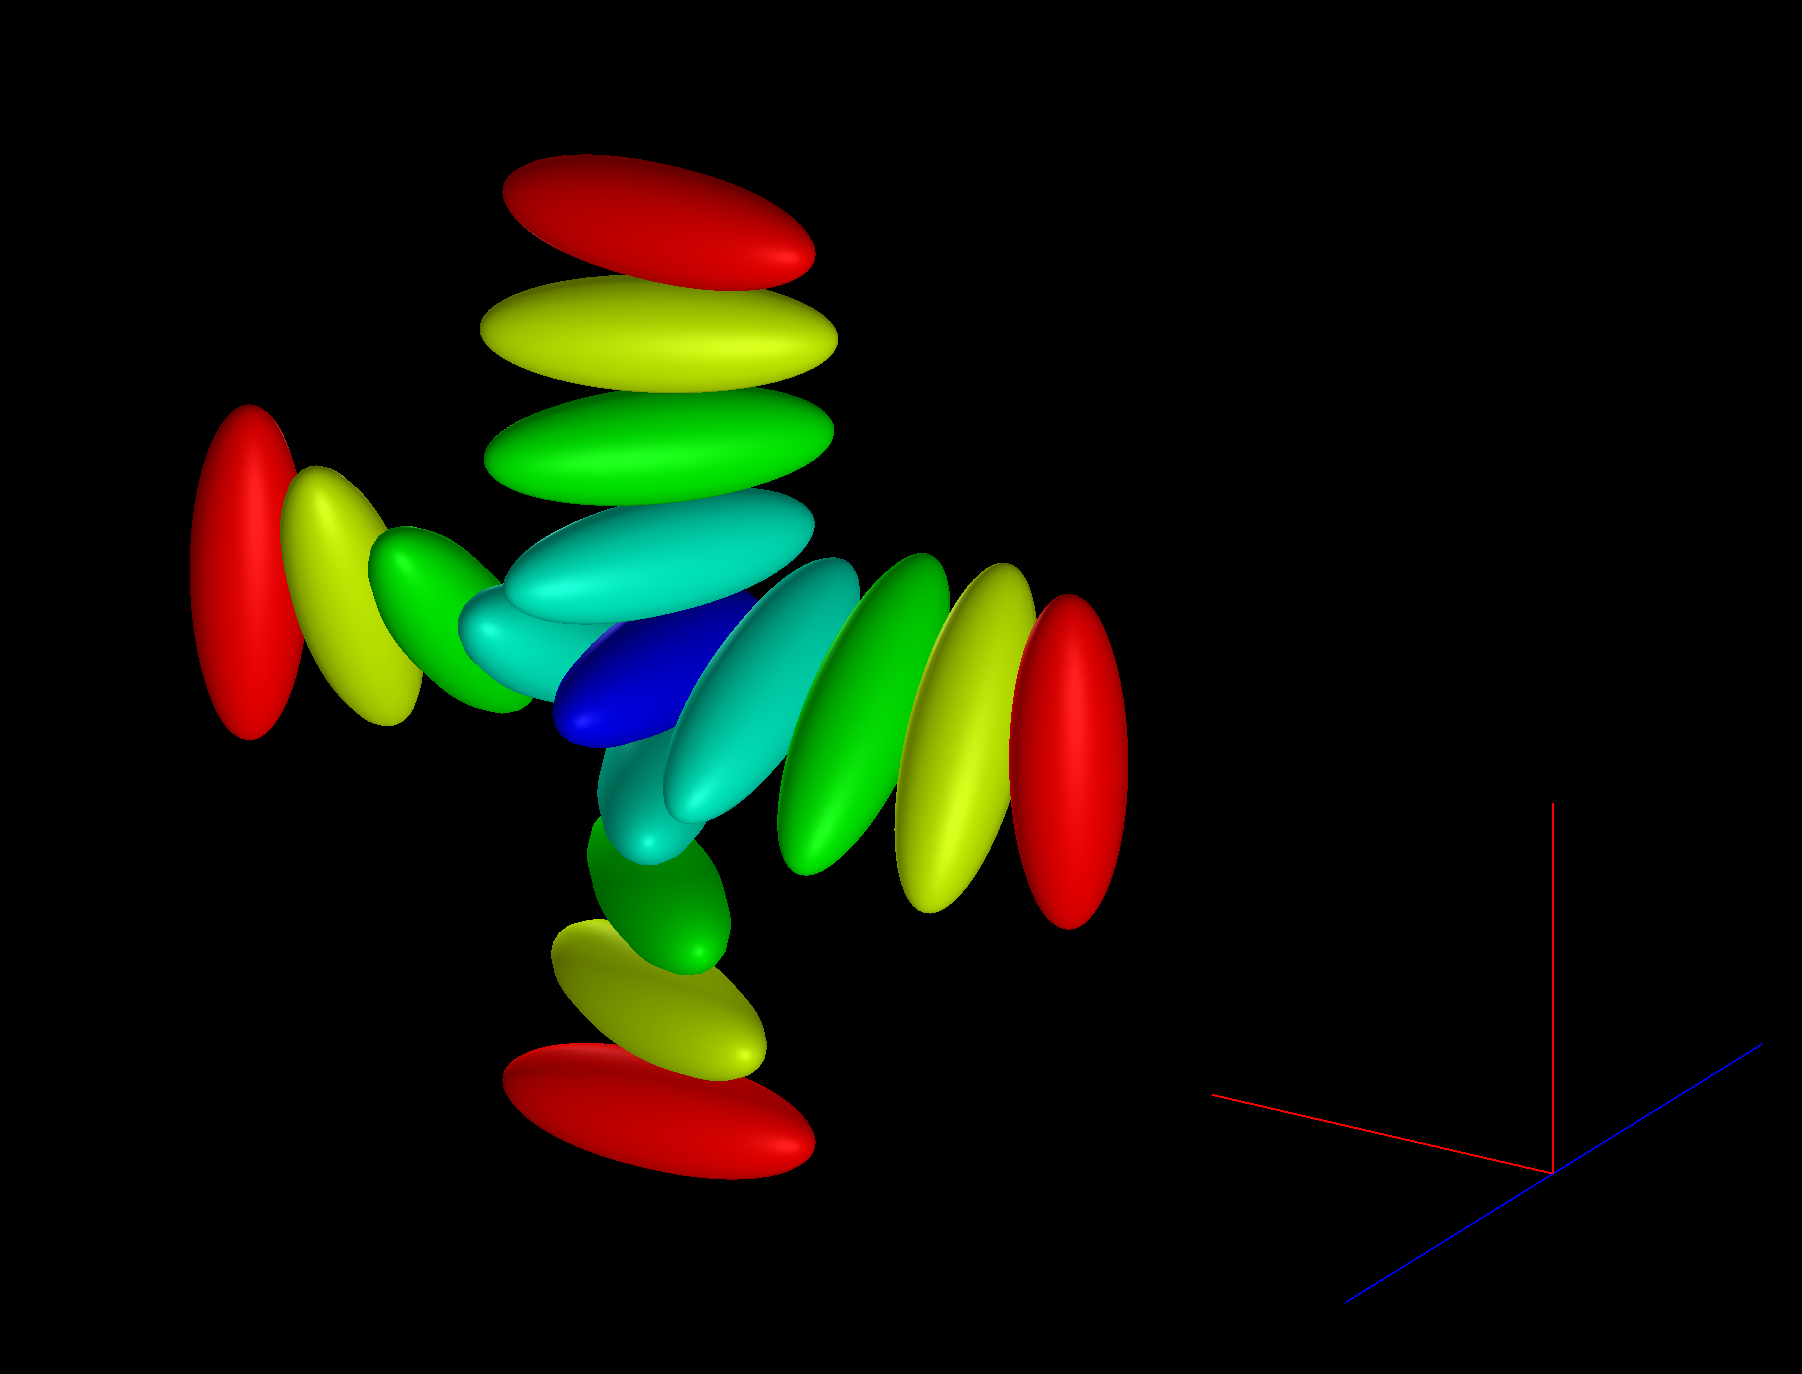
\includegraphics[width=\linewidth]{assets/images/axes/2_new_1}
      \caption{}
      \label{fig:2_new_1}
    \end{subfigure}
    \begin{subfigure}{0.4\textwidth}
      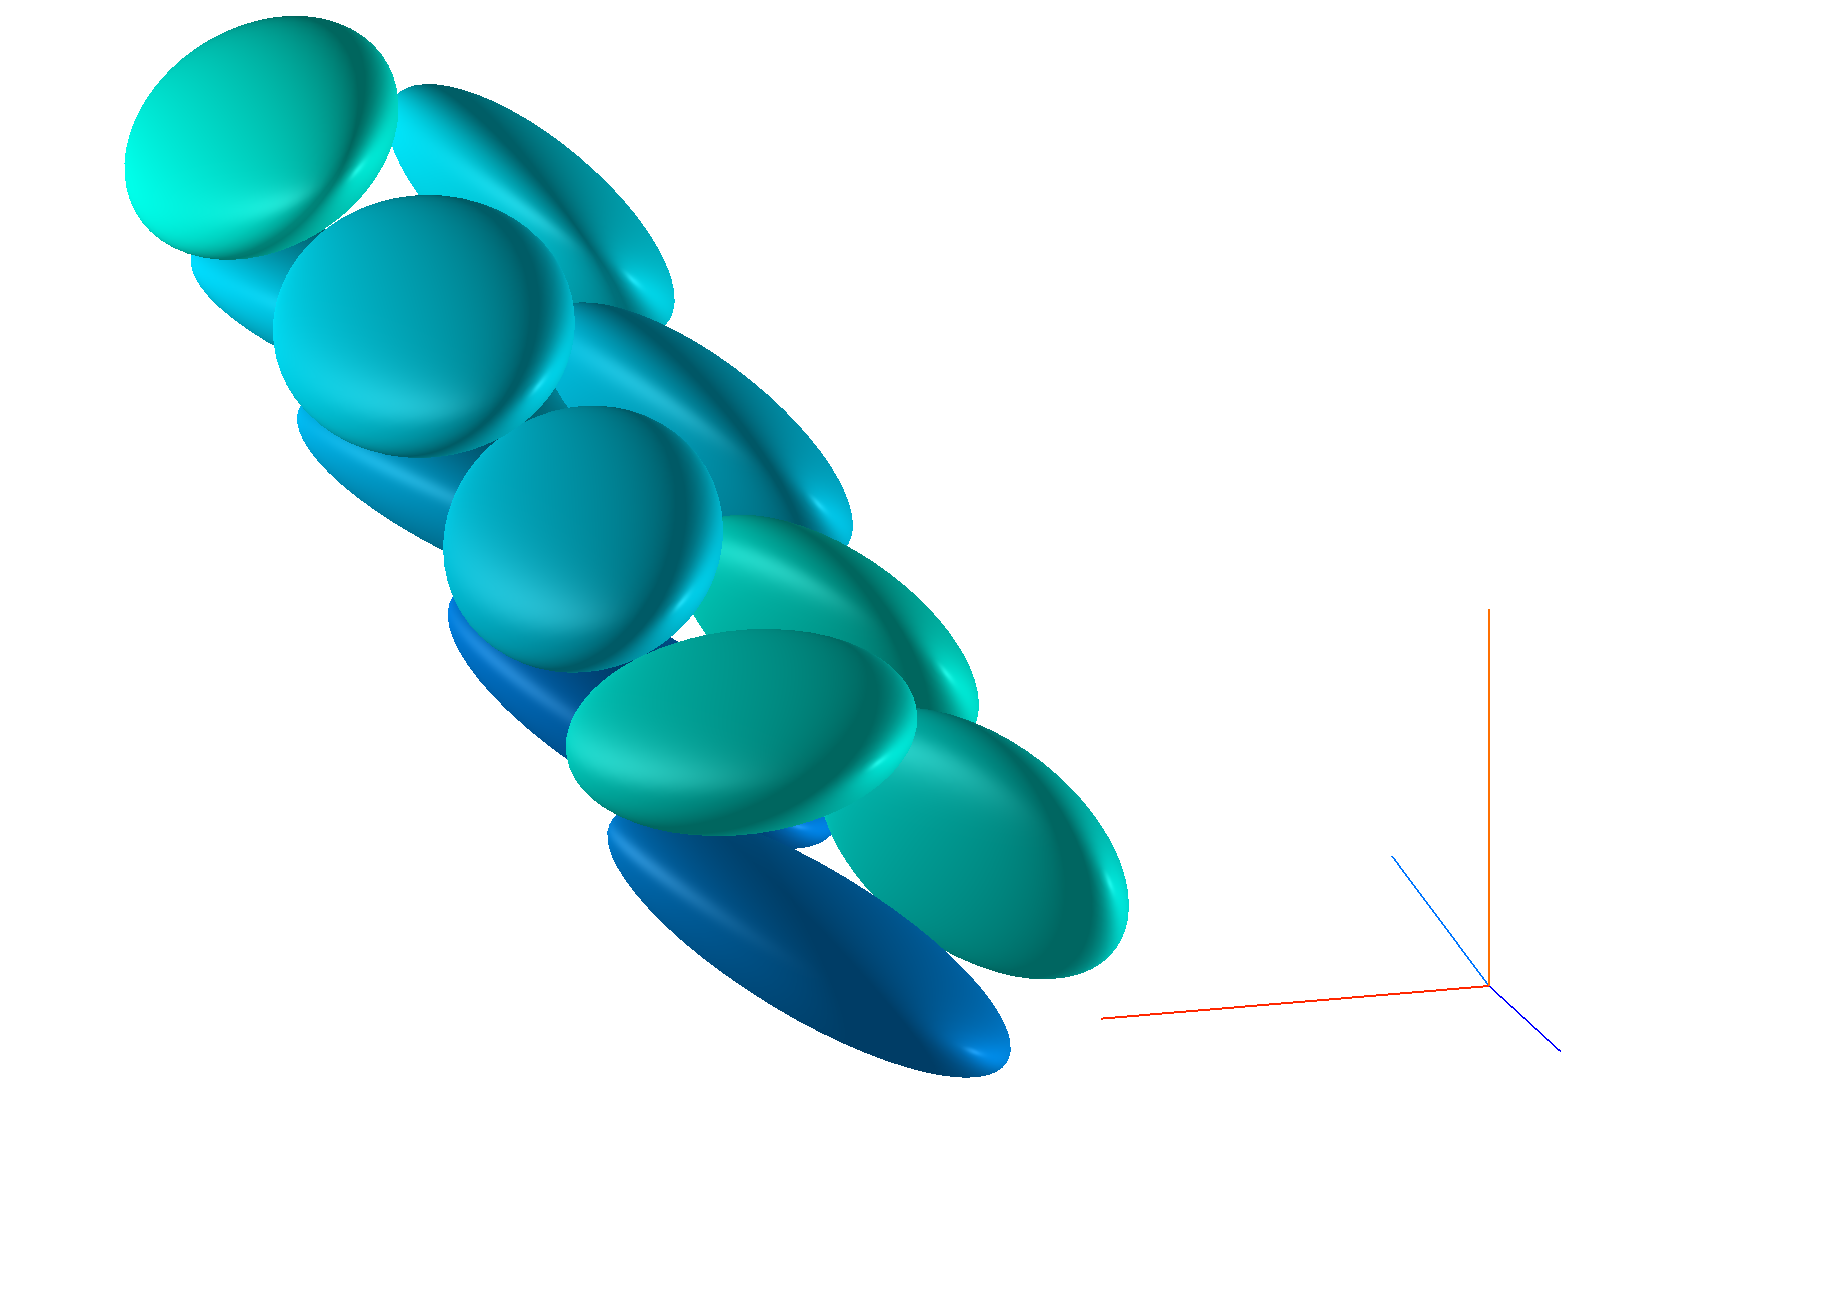
\includegraphics[width=\linewidth]{assets/images/axes/2_new_2}
      \caption{}
      \label{fig:2_new_2}
    \end{subfigure}
  \end{center}
  \caption{Axes in WebMGA 3.0.}
  \label{fig:new_axes}
\end{figure}

Some result can be viewed in \cref{fig:new_axes}.

\subsection{WebMGA 3.0 Bugs}
The axes are currently lacking labels which would be useful for identifying their intended. Ideally, the end of each axis line should have a letter indicating $x$, $y$, $z$, or $\mathbf{n}$ (for the director).
